\centering
\begin{tabular}{ll}\small
% line 1
\begin{lstlisting}[mathescape,escapechar=\#]
assume (f_compute f_emu) =  gpmem( f)
sample (f_emu( array( -20, $\cdots$, 20)) 

             #\raisebox{-0.2\height}{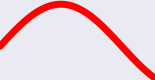
\includegraphics[height=.5cm]{figs/oneline.png}}# $\sim \mathcal{N}(\mu,\mathbf{K})$
\end{lstlisting}
& \raisebox{-0.5\height}{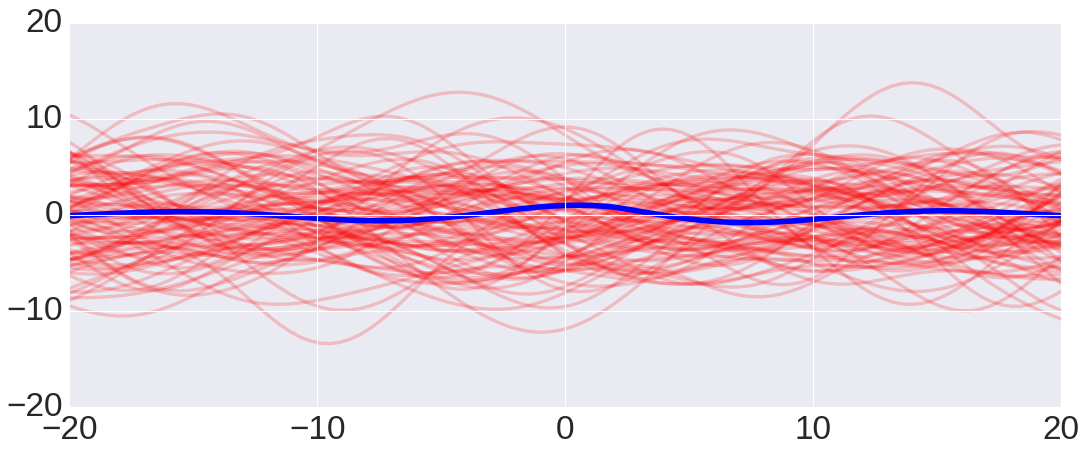
\includegraphics[height=2.5cm]{figs/slide1_0pred.png}} \\ \hline
% line 2
\begin{lstlisting}[mathescape,escapechar=\#]
predict f_compute( 12.6)

sample (f_emu( array( -20, $\cdots$, 20)) 

\end{lstlisting}
 &  \raisebox{-0.5\height}{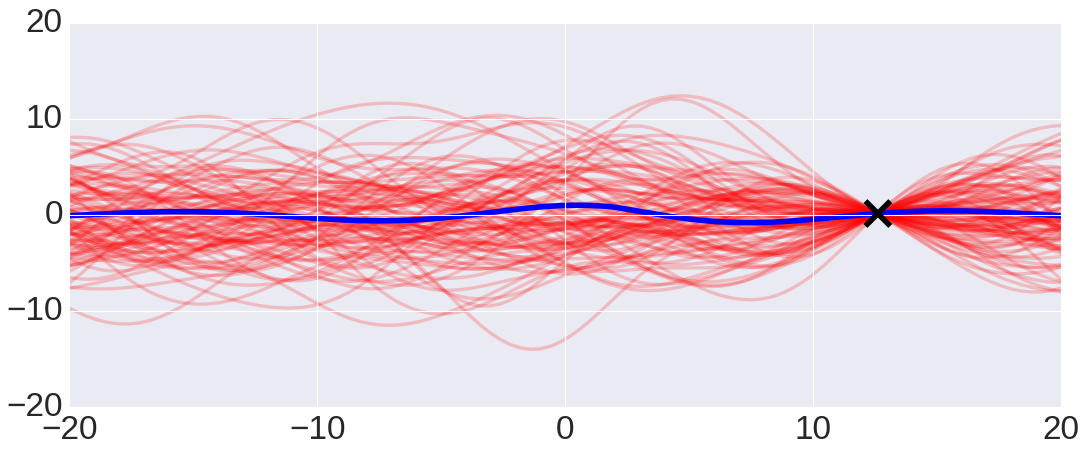
\includegraphics[height=2.5cm]{figs/slide1_1pred.png}}  \\ \hline
% line 3
 \begin{lstlisting}[mathescape,escapechar=\#]
predict f_compute( -6.4)

sample (f_emu( array( -20, $\cdots$, 20)) 
  
\end{lstlisting}
 &   \raisebox{-0.5\height}{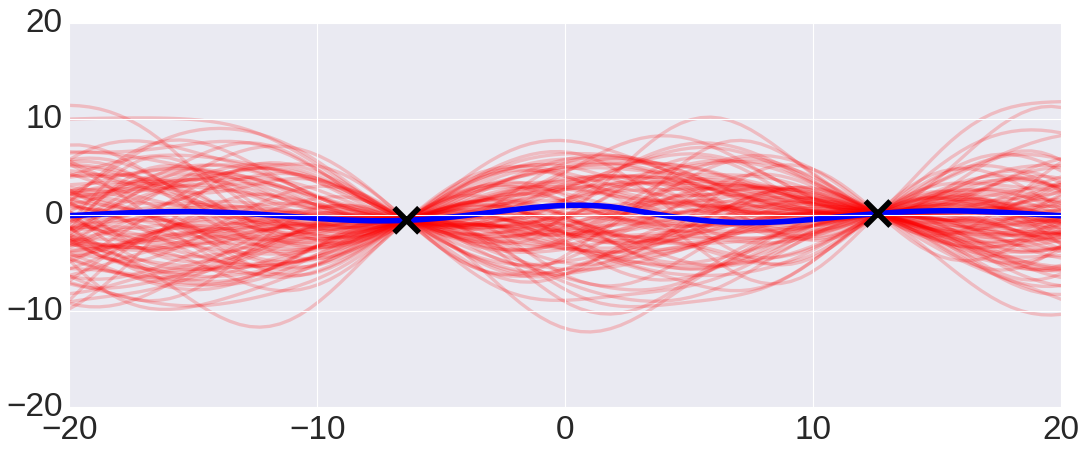
\includegraphics[height=2.5cm]{figs/slide1_2pred.png}}
\end{tabular}